\section{Evaluation}
\label{sec:evaluation}
To evaluate the performance of \name, we have conducted extensive experiments using real-world data collected from \textcolor{red}{some well-known companies}. Firstly we introduce the data set (Section~\ref{subsec:datasets}) and metrics (Section~\ref{subsec:evaluation_metrics}) used for evaluation experiments. Secondly, we introduce baseline methods briefly in (Section~\ref{Baseline methods}) and our experimental settings are recommended in (Section~\ref{Experimental settings}).
Thirdly, we compare the performance of \name{} with supervised learning based method (Opprentice), unsupervised learning based method (Donut), semi-supervised learning based method (ADS) as well as a widely used method called ATAD (Section~\ref{Evaluation of the Overall Performance}). After that, to highlight the importance of active learning and our selection strategy, we compare \name{} with its variants without active learning and another selection strategy (Section~\ref{subsec:Different_Active_Learning}). Finally, to evaluate the importance of clustering, we designed two methods without using clustering for comparison experiments (Section~\ref{subsec:whether-clustering}).

\subsection{Experimental Design}
\label{Experimental design}

\subsubsection{Data Set}
\label{subsec:datasets}

\textcolor{red}{We select 126 real KPI streams from well-known companies for clustering and 80 KPI streams as newly emerging data for anomaly detection. The information of these KPI streams is shown in Table~\ref{table:KPI streams}.}

\begin{table*}
\caption{126 KPI streams for clustering and 80 KPI streams as newly emerging data set for anomaly detection.}
\label{table:KPI streams}
\begin{center}
\begin{tabular}{| c | c | c | c |}
\hline
\textbf{Process} & \textbf{number of KPI streams} & \textbf{Interval (minute)} & \textbf{Length (month)} \\ \hline
Clustering & 126 & 5 &	1 \\ \hline
Anomaly Detection & 80 & 5 &	1 \\ \hline
\end{tabular}
\end{center}
\vspace{0 mm}
\end{table*}

In \name{}, we first apply ROCKA~\cite{lirobust} to cluster all the 126 historical/existing KPI streams into \textcolor{red}{9} clusters. In order to verify the accuracy of ROCKA clustering, we ask experienced operators to manually group the 126 KPI streams according to their shape. We find that ROCKA is basically able to group all the 126 historical/existing KPI streams into the right cluster. In addition, with the help of ROCKA's preprocessing and SBD distance,we successfully classifies all the 80 new KPI streams into the correct cluster.

To evaluate the performance of anomaly detection methods, operators manually label several anomalous data points of the 9 cluster centroids obtained by ROCKA randomly. And the new 80 KPI streams are used for the following evaluation experiments. Therefore, there is no need to manually labeling the remaining 117 (126 minus 9) historical/existing KPI streams. 

In summary, We have a total of 206 (126 plus 80) time series, and 80 of which are used for evaluation. We believe that the 206 KPI streams are sufficient to evaluate \name{}'s performance.

\subsubsection{Evaluation Metrics}
\label{subsec:evaluation_metrics}
We use a simple strategy following~\cite{xu2018unsupervised}, if we select a threshold, any point in an abnormal segment in the ground truth can be detected, it is said that the abnormal segment is correctly detected, and all points in this segment are considered to be detectable by this threshold. At the same time, the points outside the abnormal segment are treated as normal. The precision, recall, F-score, and best F-score are then computed accordingly.

% \begin{figure}
%       \begin{minipage}[h]{1.0\linewidth}
%       \centering
%       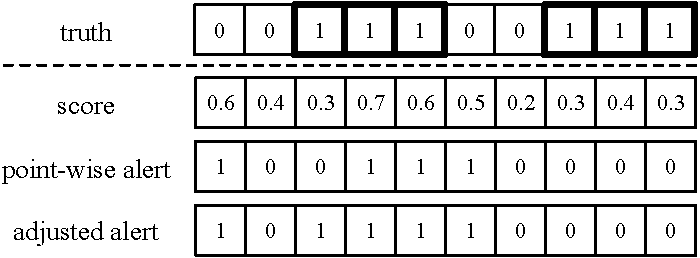
\includegraphics[width=0.9\textwidth]{fig/label_calculate.pdf}\\
%       \end{minipage}
%       %\vspace{-5 mm}
%       \caption{Illustration of the strategy for modified metrics. The first row is the truth with 10 contiguous points and two anomaly segments highlighted in the shaded squares. The detector scores are shown in the second row. The third row shows the point-wise detector results with a threshold of 0.5. The fourth row shows the detector results after adjustment. We shall get precision 0.6, and recall 0.5. From the third row, the alert delay for the first segment is 1 interval (5 minutes)~\cite{xu2018unsupervised}.}
%       \label{fig:label_calculate}
% \end{figure}

F-score is commonly used as an evaluation to build up the balance of precision and recall~\cite{atad}. To obtain the best possible performance of an anomaly detection method on a particular testing set, we apply the \emph{best F-score} as the metric to evaluate anomaly detection methods.

Note that in Section~\ref{Evaluation of the Overall Performance}, we use the \emph{best F-score} to evaluate the anomaly detection on the testing set (namely, the back 60\% of every new KPI stream). Although it is not entirely practical in real-world applications, it fully compares the best performance of \name{}, Opprentice, Donut, ADS, and ATAD.

\subsubsection{Baseline Methods}
\label{Baseline methods}
In order to examine the performance of our proposed method, we selected several commonly-used anomaly detection algorithms as baseline methods. 
\begin{itemize}
\item
  In order to compare our framework \name{} with supervised based methods, we chose Opperentice~\cite{liu2015opprentice} as a baseline method. A supervised based method aims to build an anomaly detection for normal and anomalous classes. Every point in KPI streams is labeled by operators. Opperentice uses the labels on anomalies to train a random forest classifier and does not require manual selection of parameters and adjustment of thresholds.
  \item 
  In order to compare our framework \name{} with unsupervised based methods, we chose Donut~\cite{xu2018unsupervised} as a baseline method. Donut is an unsupervised anomaly detection algorithm based on VAE (Variational Auto-Encoder) for seasonal KPIs with local variations. Donut can work when there are no labels of KPI streams at all.
  \item  
  In order to compare our framework \name{} with semi-supervised based methods, we chose ADS~\cite{ADSarticle} as a baseline method, which is the first framework that applied semi-supervised learning to KPI anomaly detection. Through clustering and semi-supervised learning, ADS enables the rapid deployment of anomaly detection models (say at most 3 weeks) for a large number of emerging KPI streams, without manual algorithm selection, parameter tuning, or new anomaly labeling for emerging KPI streams. 
  \item 
  On the basis of semi-supervised learning, in order to compare our framework \name{} with a method which also reduces the amount of labeling, we select ATAD~\cite{atad} as another baseline method. It combines transfer learning and active learning and could achieve a balance between labeling effort and performance. In transfer learning, ATAD transfers the common anomalous behavior learned from a labeled KPI stream to a large volume of target unlabeled data set to reduce the labeling effort for the target data set. In active learning, ATAD improves the detection performance by labeling only a small number of selected samples in the target data set. 
  

\end{itemize}

\subsubsection{Experimental Settings}
\label{Experimental settings}
\par
During our experiment, we set some parameters for our data set.
\par
For extracting the temporal features, we set the length of sliding window $w$ as 6. As for the forecasting error features, we set $w$ as 30 for Holt and twice the period $p$ for Holt-winters and STL, because we have to reduce the window length as much as possible to meet the requirements of rapid deployment.
\par
For the PU learning, $s\%$ is the ratio of initial negative samples ($setN$) selected from unlabeled samples ($setU$). $p\%$ is the ratio of samples selected from unlabeled samples ($setU$) during self-training step. As a matter of experience, we set $s\%$ as 20\% and $p\%$ as 70\%. Because in the pre-training step, if we choose too many negative samples from $setU$, we might get some positive samples mixed in $setN$, which could cause the final model to perform poorly. As for the self-training step, because we adopt active learning to label some possible $P$, the reliability of the model is high, thus we can select more samples during this step. During the self-training step, We set the positive class prior $\pi$ as 0.015, though we estimate it to 0.01. Because during active learning, we discover that not all the possible positive samples are positive in fact. To find as many positive samples as possible, we set the positive class prior $\pi$ much bigger. And we set speed $K$ as 200, because we want to find reliable positive samples in every iteration.

\begin{table*}
\caption{The comparison of the F-score in 9 clusters using three different methods in the PU learning process, including without active learning, label classification boundaries when active learning and label possible P when active learning.}
\label{table:difference_active}
\begin{center}
\begin{tabular}{| c | c | c | c |}
\hline
\textbf{Clusters$\backslash$F-score} & \textbf{Without active learning} & \textbf{Label classification boundaries} & \textbf{Label possible P} \\ \hline
1 & 0.612	& 0.812 &	0.923 \\ \hline
2 & 0.545	& 0.667 &	0.967 \\ \hline
3 & 0.819   & 0.860 &   0.878 \\ \hline
4 & 0.745   & 0.860 &	0.868 \\ \hline
5 & 0.596   & 0.785 &	0.839 \\ \hline
6 & 0.458	& 0.638 &   0.742 \\ \hline
7 & 0.871   & 0.872 &	0.926 \\ \hline
8 & 0.714	& 0.793 &   0.823 \\ \hline
9 & 0.587   & 0.673 &	0.704 \\ \hline
Average & 0.636 & 0.772 & 0.840 \\ \hline
Increase ratio & 32.1\% & 8.7\% & --\\ \hline
\end{tabular}
\end{center}
\vspace{0 mm}
\end{table*}

\subsection{Evaluation of the Overall Performance}
\label{Evaluation of the Overall Performance}
To our knowledge, this is the first work to apply PU learning and active learning to time series anomaly detection problems. In order to evaluate the performance of \name{}, we calculate its best F-score, and compare it with that of Opperentice~\cite{liu2015opprentice}, ADS~\cite{ADSarticle}, Donut~\cite{xu2018unsupervised} as well as ATAD~\cite{atad}.


\textcolor{red}{In \name{}, for each of the 80 new KPI streams, classifier them into the correct cluster firstly. Then, extract the features of time series to convert data points into a set of feature vectors. To ensure the consistency of the data sets in each baseline, we combine the former 40\% of each new KPI stream with its partially labeled cluster centroid after the PU learning, and train a detection model together.} 
% For each of the 80 new KPI streams, We train \name{} with the features extracted from the first 20\% of it and the 2 anomalous points randomly manual labels, as well as the features of its cluster centroid (KPI stream) and the 8 anomalous points randomly manual labels, then use \name{} to detect anomalies on the back 60\% of these new KPI stream. The reason why we chose the back 60\% of each new KPI stream instead of the back 80\% as the test set is that in the comparison method ADS, the first 20\% of each new KPI stream is used for random manual labeling, and then 20\% to 40\% of it is needed for semi-supervised learning. Therefore, in order to ensure the consistency of the training data set, we use all these models to detect anomalies on the back 60\% of each of the 80 new KPI streams.

\begin{figure}
  \begin{minipage}{1.0\linewidth}
  \centering
  %\setlength{\abovecaptionskip}{3.cm}
  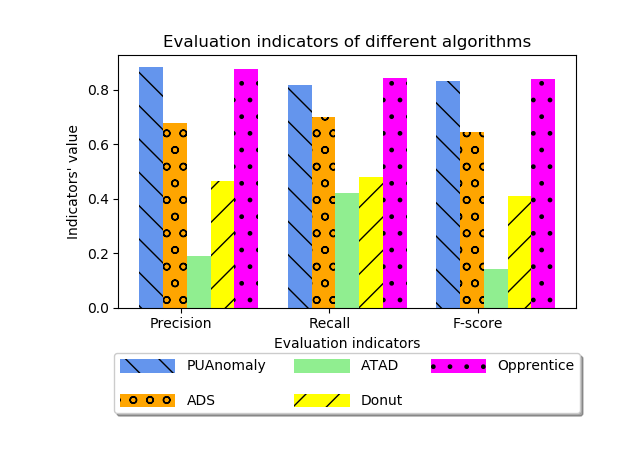
\includegraphics[width=0.9\textwidth]{ADS_Journal/PU figures/change_1.png}\\
  \end{minipage}
  \caption{The Evaluation indicators of different detectors.}
  \label{fig:Evalution indicators}
\end{figure}

Figure~\ref{fig:Evalution indicators} shows the average precision, recall, and best F-score of all the 80 new KPI streams using the above five methods. We can see that both \name{} and Opperentice perform superior in detecting anomalies for KPI streams, with the average best F-score of 0.833 and 0.840, respectively. In contrast, ADS performs a little worse than them whose average best F-score of all new KPI streams is 0.647. The performance of the above three models is much better than that of ATAD and Donut, for the following reasons:
(1) ATAD (Active Transfer Anomaly Detection) extract features from all KPI streams, cluster labeled data sets, then assign unlabeled data sets to existing clusters, and use transfer learning and active learning to train an anomaly detection model. Firstly, the clustering method of ATAD is based on time data points rather than time series which only pays attention to KPIs' diversity but ignores the similarity between some KPI streams. Secondly, ATAD requires that the anomaly labeling ratio of all historical/existing KPI streams is 1\% to 5\%, but the amount of manual labeling in \name{} is even less than 1\%, we suspect that too few labels will affect the effectiveness of ATAD.
(2)  Donut is a deep Bayesian model, which requires a lot of training data to get good detection results (say six months worth of KPI streams). However, we only need to train with the former 60\% of the cluster centroid, which is 18 days' data, to achieve a satisfactory result. The data set is too small for Donut, we suspect it will affect the effectiveness.

To intuitively compare the best F-scores of \name{}, Opperentice, ADS, and Donut, we draw a line graph of the average best F-scores of the above four methods on the nine clusters in Figure~\ref{fig:Average Fscore}. Because the ATAD algorithm clusters all data features, which is different from the clustering methods used in other methods, thus Figure~\ref{fig:Average Fscore} do not include ATAD. \name{} and Opperentice perform better than the other two methods on all the nine clusters. This experimental result proves that our method is significantly better than ADS, because we use active learning to check samples and ensure the correctness of labeled anomalous samples.

It can be seen that the F-score in each cluster of \name{} is close to the F-score of Opperentice. As aforementioned, new KPI streams are continuously produced in Internet-based services thus the number is gradually increasing. Manually labeling all the newly emerging KPI streams to detect KPI anomalies is infeasible in practice. Therefore, supervised based methods are not appropriate for our scenario.

\begin{figure}
  \setlength{\belowcaptionskip}{0cm}
  \begin{minipage}[H]{1.0\linewidth}
  \centering
  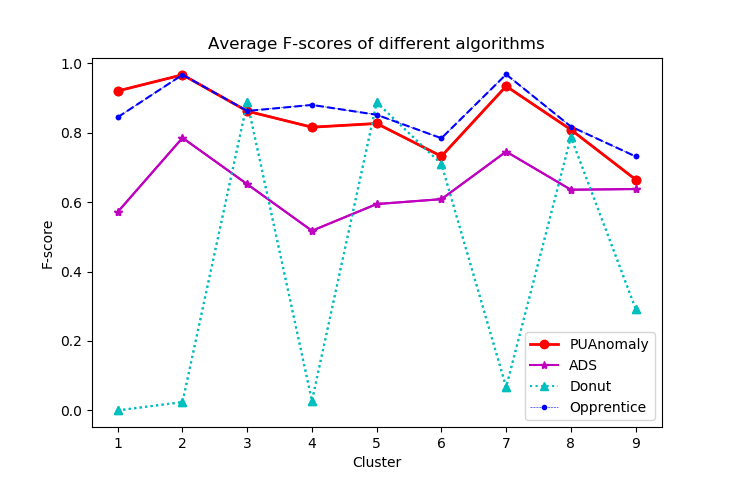
\includegraphics[width=0.9\textwidth]{ADS_Journal/PU figures/myplot2.png}\\
  \end{minipage}
  \caption{The Average F-scores of different clusters.}
  \label{fig:Average Fscore}
%   \vspace{0 mm}
\end{figure}


\subsection{Evaluation of the Novel Active Learning Component}
\label{subsec:Different_Active_Learning}

To the best of our knowledge, many selection strategies have been proposed for traditional active learning. 
% In the field of time series anomaly detection, selecting the samples at classification boundaries to label is widely used now. 
As aforementioned, 
% when algorithm iteratively selecting credible anomalous samples for labeling, such a strategy allows us to choose the samples on the classification boundaries to label firstly. However, if a normal sample is similar to an anomalous sample, it will appear at the classification boundary, causing the algorithm to classify it as an anomalous by mistake. Then due to the similarity between normal samples, resulting in more and more normal samples being incorrectly labeled as anomalous samples. Finally, the result of detection will poor. To solve this problem above, we adopted another selection strategy. 
we select the samples that may be anomalous instead of the samples at the classification edge to label. In this way, we avoided misclassification and the labeling result is more accurate. In order to evaluate the effectiveness of active learning especially our selection strategy, we conducted a comparative experiment of active learning to compare the algorithm that does not use active learning with the algorithm that labels edge samples for classification and the algorithm that labels may be normal examples.

\begin{figure}
  \setlength{\belowcaptionskip}{-0.2cm}
  \begin{minipage}[H]{1.0\linewidth}
  \centering
  %\setlength{\abovecaptionskip}{3.cm}
  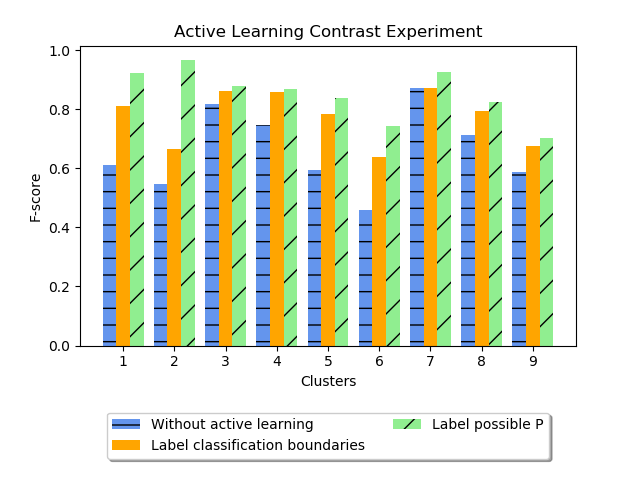
\includegraphics[width=0.9\textwidth]{ADS_Journal/PU figures/active_update.png}\\
  \end{minipage}
  \caption{The comparison among algorithm without active learning and labeling classification boundaries as most active learning algorithms and labeling the samples most likely to be normal in this paper.}
  \label{fig:whether_active_or_not}
%   \vspace{0 mm}
\end{figure}


TABLE~\ref{table:difference_active} lists the best F-score in the nine clusters when adopted different selection strategies and directly removed active learning in \name{}. For better visualization, we displayed the contents of the TABLE~\ref{table:difference_active} through a bar chart shown in Figure~\ref{fig:whether_active_or_not}.

By comparing not using active learning and our algorithm, we can see that using active learning can improve performance obviously. Moreover, we find that labeling samples at the classification boundary are almost indistinguishable from the performance without active learning. Therefore, 
our selection strategy in active learning guarantees the credibility of the selected samples for labeling, makes the addition of active learning more helpful, and achieves very good performance.

\subsection{Evaluation of Clustering}
\label{subsec:whether-clustering}
As mentioned before, there are millions of KPI streams for real-time monitoring of Internet-based services. The reason why \name{} use clustering to preprocess the historical/existing KPI streams as the first step is due to the following two considerations:
(1) If we trained only one model for all KPI streams, the detect result will be very inaccurate due to the diversity of KPI streams.
(2)If we trained an anomaly detection model separately for each KPI streams, the overhead of anomaly detection is huge when facing large-scale data.

\begin{figure}
  \begin{minipage}[h]{1.0\linewidth}
  \centering
  %\setlength{\abovecaptionskip}{3.cm}
  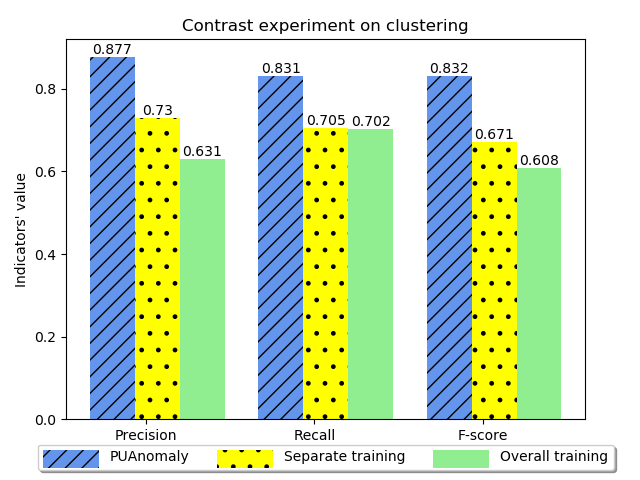
\includegraphics[width=0.9\textwidth]{ADS_Journal/PU figures/clustering with hatch.png}\\
  \end{minipage}
  \caption{The comparison of the results using three different methods including clustering of \name{}, Separate training (train a model for each new KPI stream) and Overall training (train one model for all the new KPI streams) in the clustering process.}
  \label{fig:whether_clustering_or_not}
\end{figure}

\name{} apply ROCKA~\cite{lirobust} to group the 126 historical/existing KPI streams into nine clusters, and classify 80 new KPI streams into these clusters. 
In order to verify the effect of clustering and ensure that the data set is used as consistently as possible, we adopt the following two methods compared with the method using clustering:
\begin{itemize}
  \item  
  Only train one model for all the new KPI streams. We randomly select 9 (consistent with the number of clusters in \name{}) of all historical/existing KPI streams as the training set, and 80 new KPI streams for anomaly detection, called "overall\_training". For each KPI stream of the 80 new KPI streams, we randomly select one of the 9 streams together with the former 40\% of it as the training set, and the latter 60\% of it as the testing set.
  \item 
  Train a model for each new KPI stream separately. We utilize the former 40\% of every KPI stream of the 80 new KPI streams to train a model separately, and detect the latter 60\% of it, called "separate\_training".
\end{itemize}

Figure~\ref{fig:whether_clustering_or_not} shows the best average F-score of the three methods. We find that the performance of using clustering is significantly better than the other two methods, and the efficiency is very high. Here we explain why is there such a result. 

KPI streams are diverse. If we train only one model for all KPI streams, the training set we choose may be completely different from the new KPI streams for anomaly detection. It will lead to poor detection results. Besides, if we train a separate model for each new KPI stream, it will produce a large load in actual production.

Consequently, using clustering is necessary for time series anomaly detection.

\subsection{Evaluation of Parameter}
As mentioned in \ref{Experimental settings}, there are several parameters in our framework. To evaluate the effects of these parameters on \name~, we compare the performance of \name~under different values of these parameters.
\par
In this section, we set progressive parameter levels to evaluate the correlation between parameter and model performance.
For the ratio of pre-training $s\%$, which means the proportion of labeling unlabeled samples as negative during pre-training, we set it from 0.05 to 0.4 respectively. For the speed of PU learning, we set it from 200 to 1000 respectively. For the count of initially labeling, we set it from 2 to 20 respectively.
\par
Then, we compare the performance of \name~for the parameters selected within the scope above.
From figure \ref{fig:parameters} it can be seen that \name~always has good and stable performance by using these above parameters, this to say, \name~is insensitive to these parameters.
Therefore, these parameters can be selected within the scope above.
\begin{figure}
    \centering
	  \subfloat{
	  \begin{minipage}[h]{0.5\linewidth}
      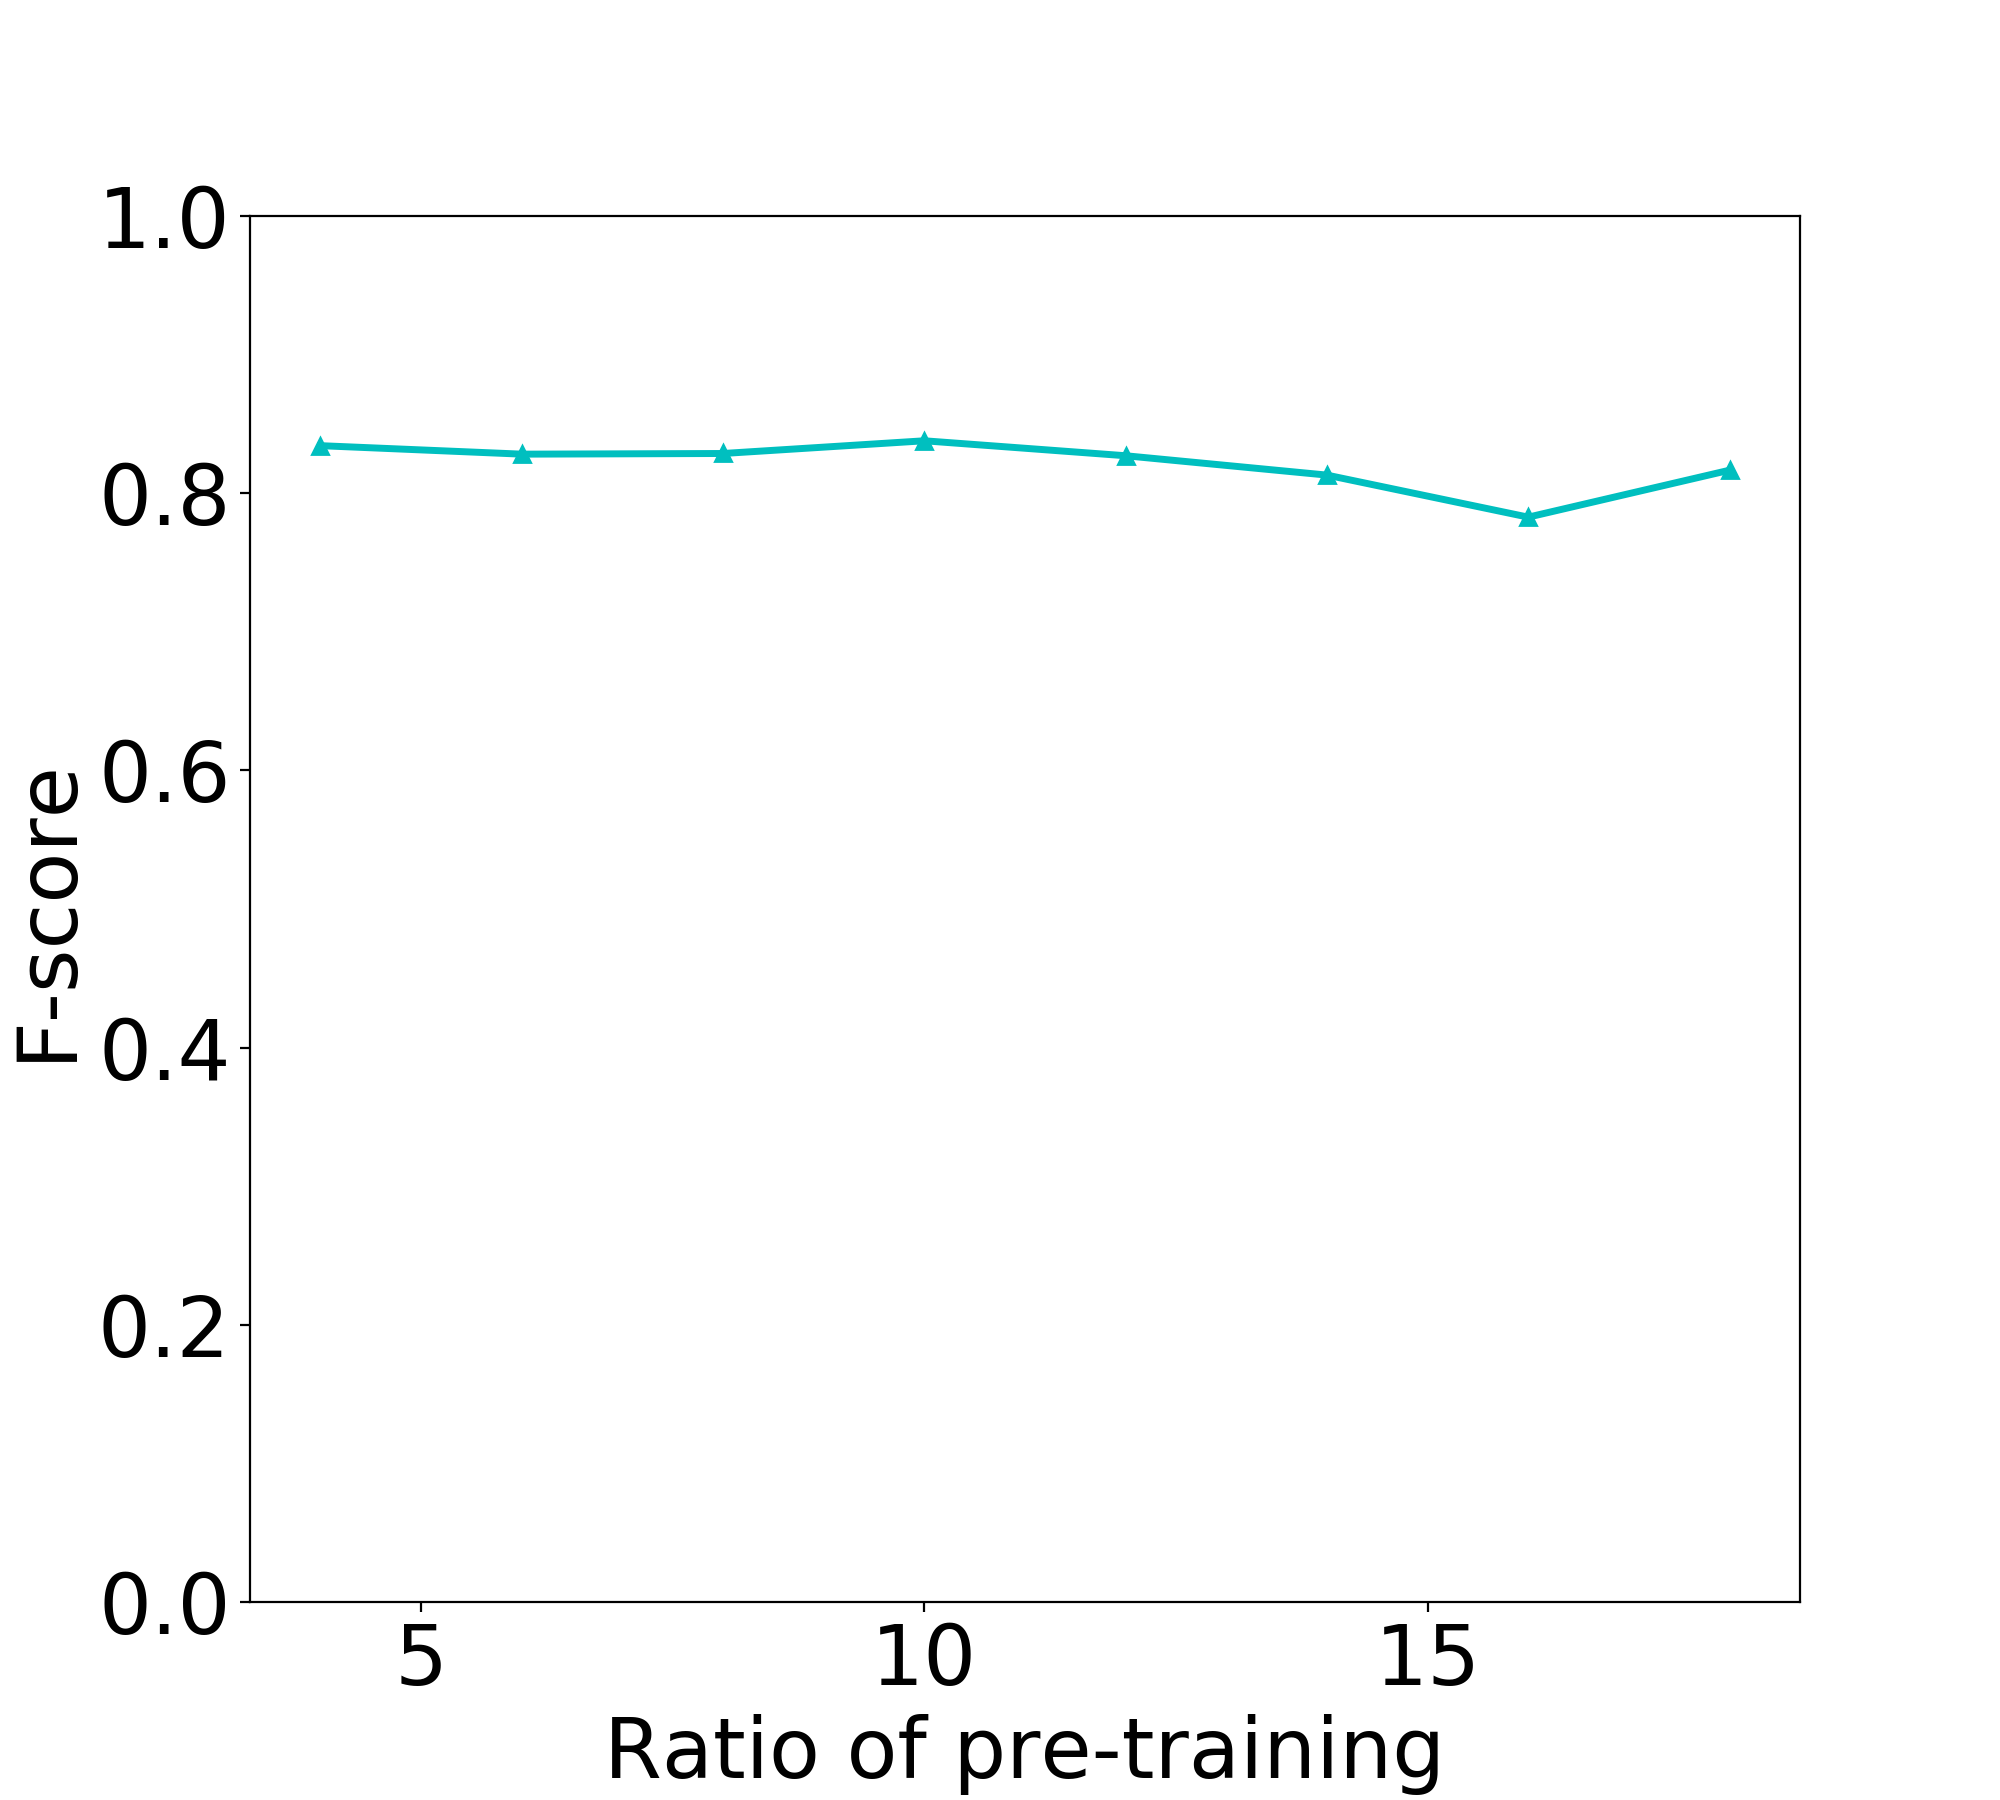
\includegraphics[width=1.1\linewidth]{ADS_Journal/PU figures/para_s.png}\label{a}
      \end{minipage}}
	  \subfloat{
	  \begin{minipage}[h]{0.5\linewidth}
      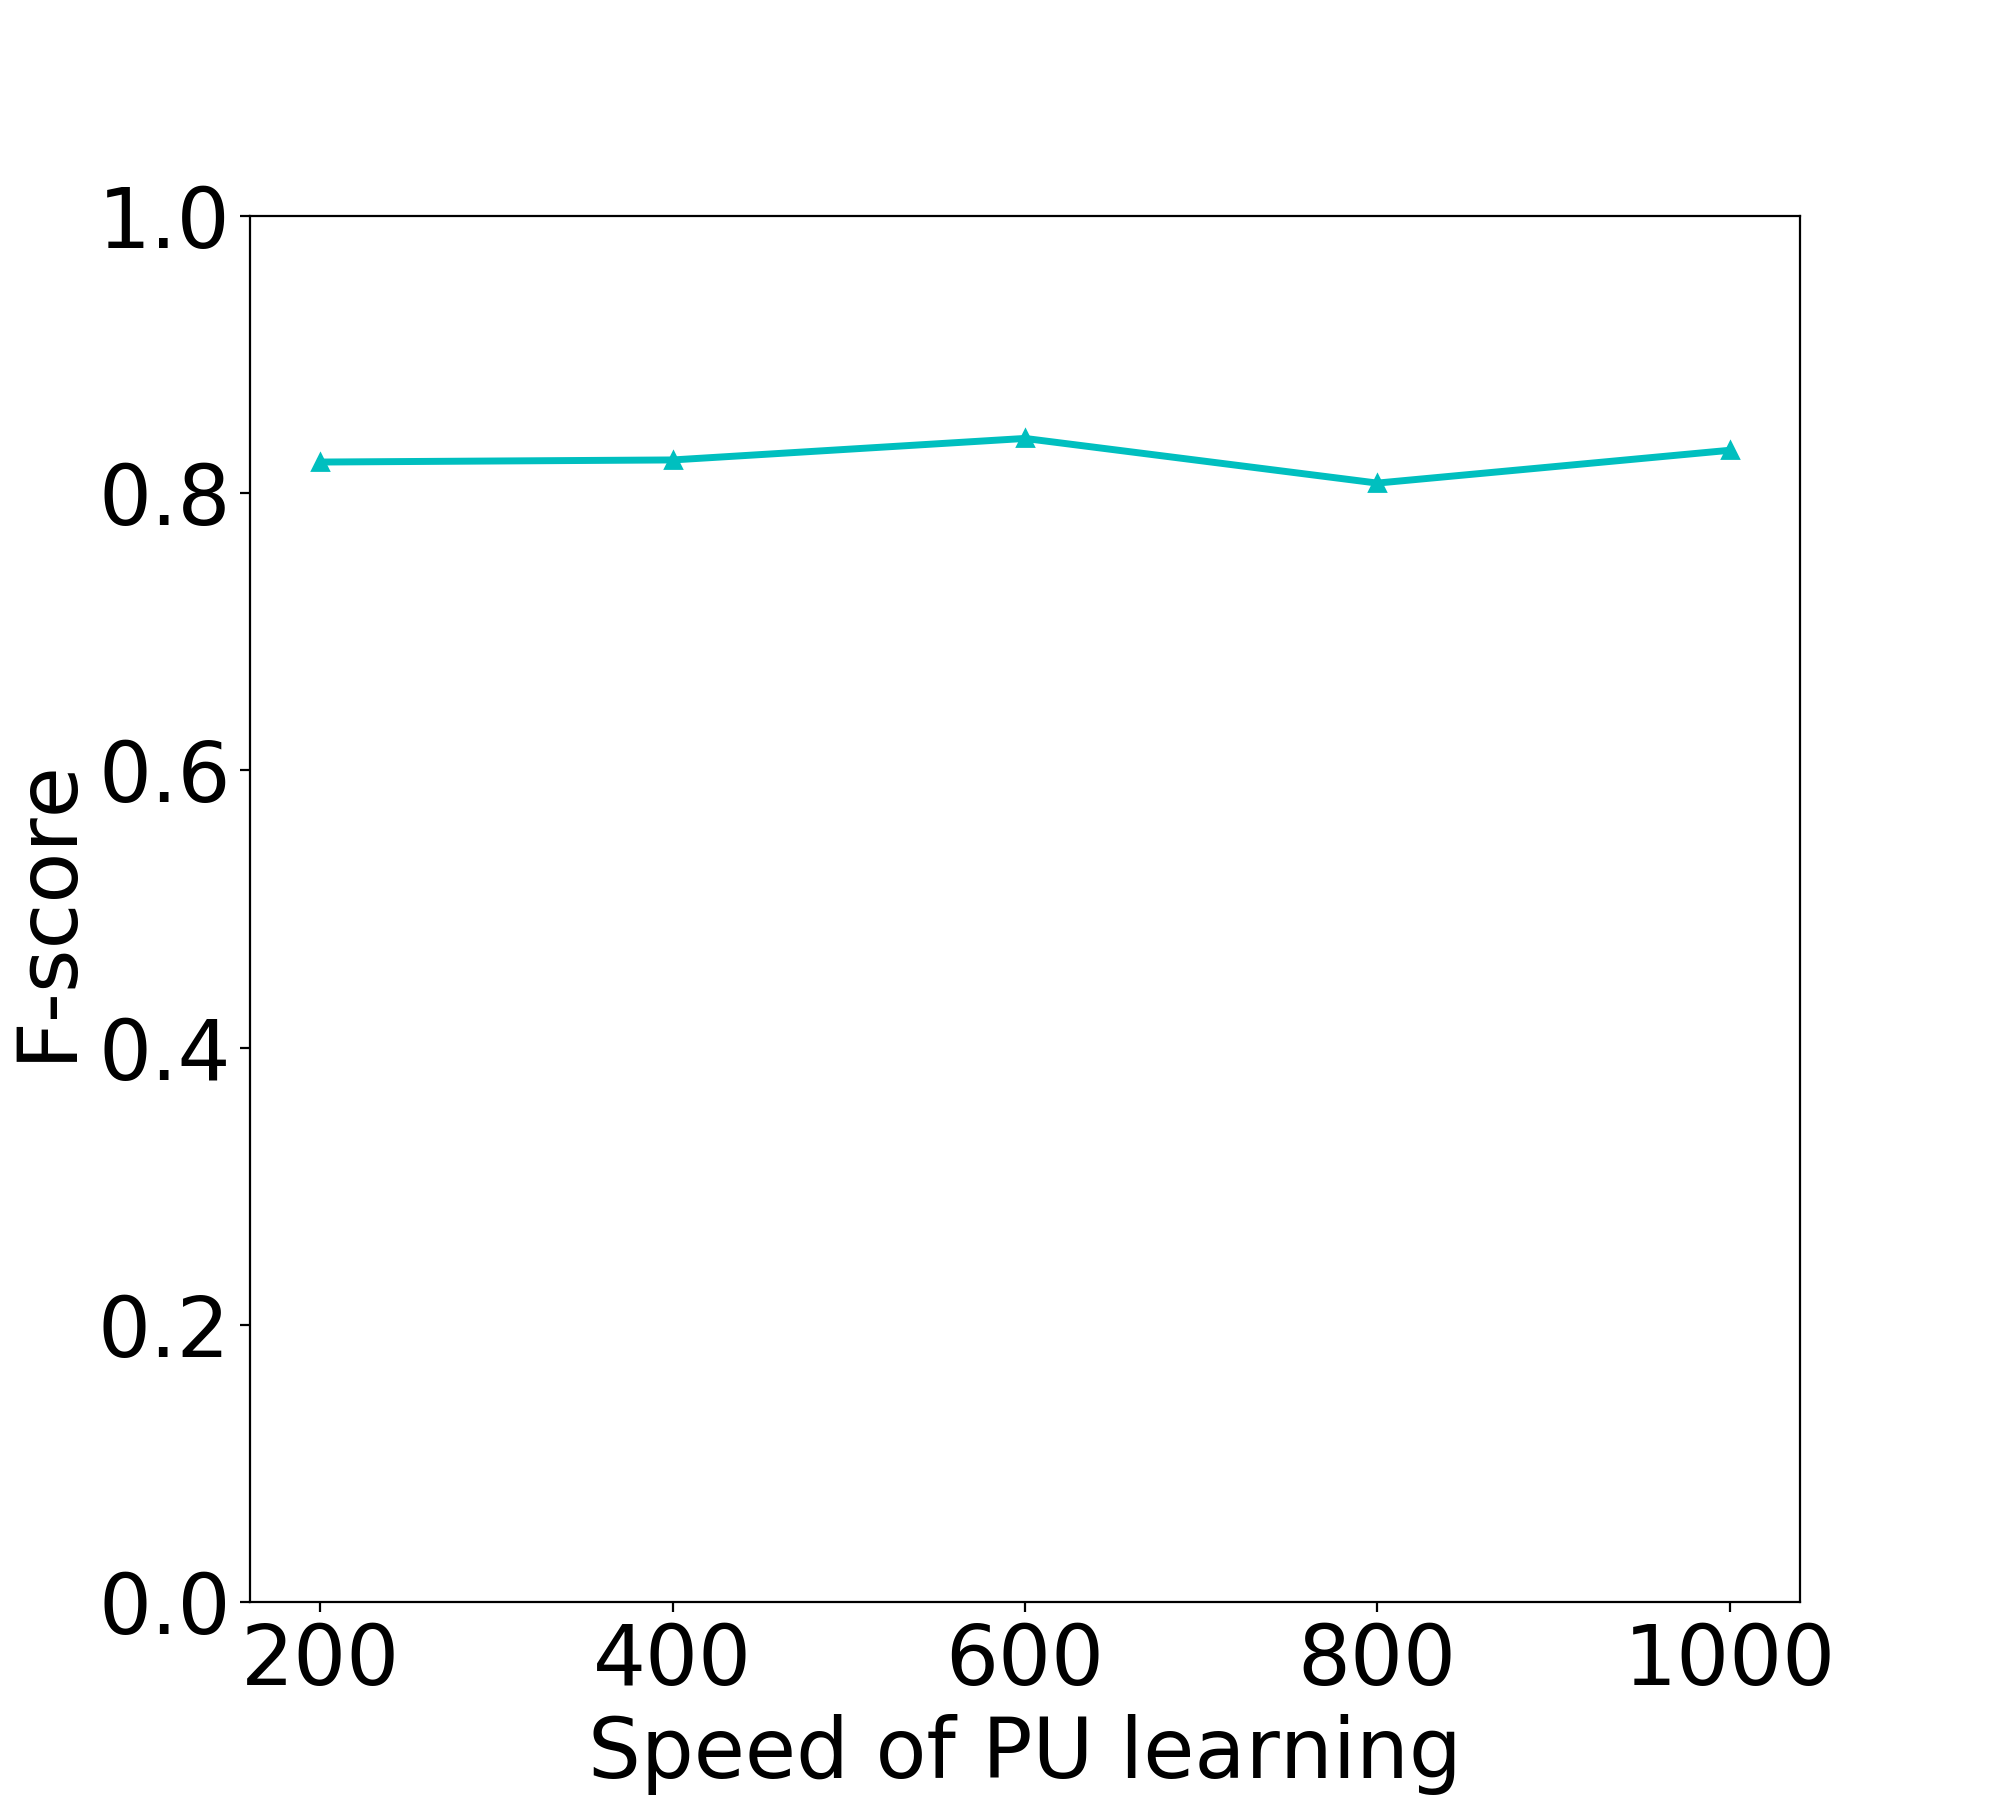
\includegraphics[width=1.1\linewidth]{ADS_Journal/PU figures/para_step_size.png}\label{b}
      \end{minipage}}
      
      \vspace{0.15in}
	  \subfloat{
	  \begin{minipage}[h]{0.5\linewidth}
      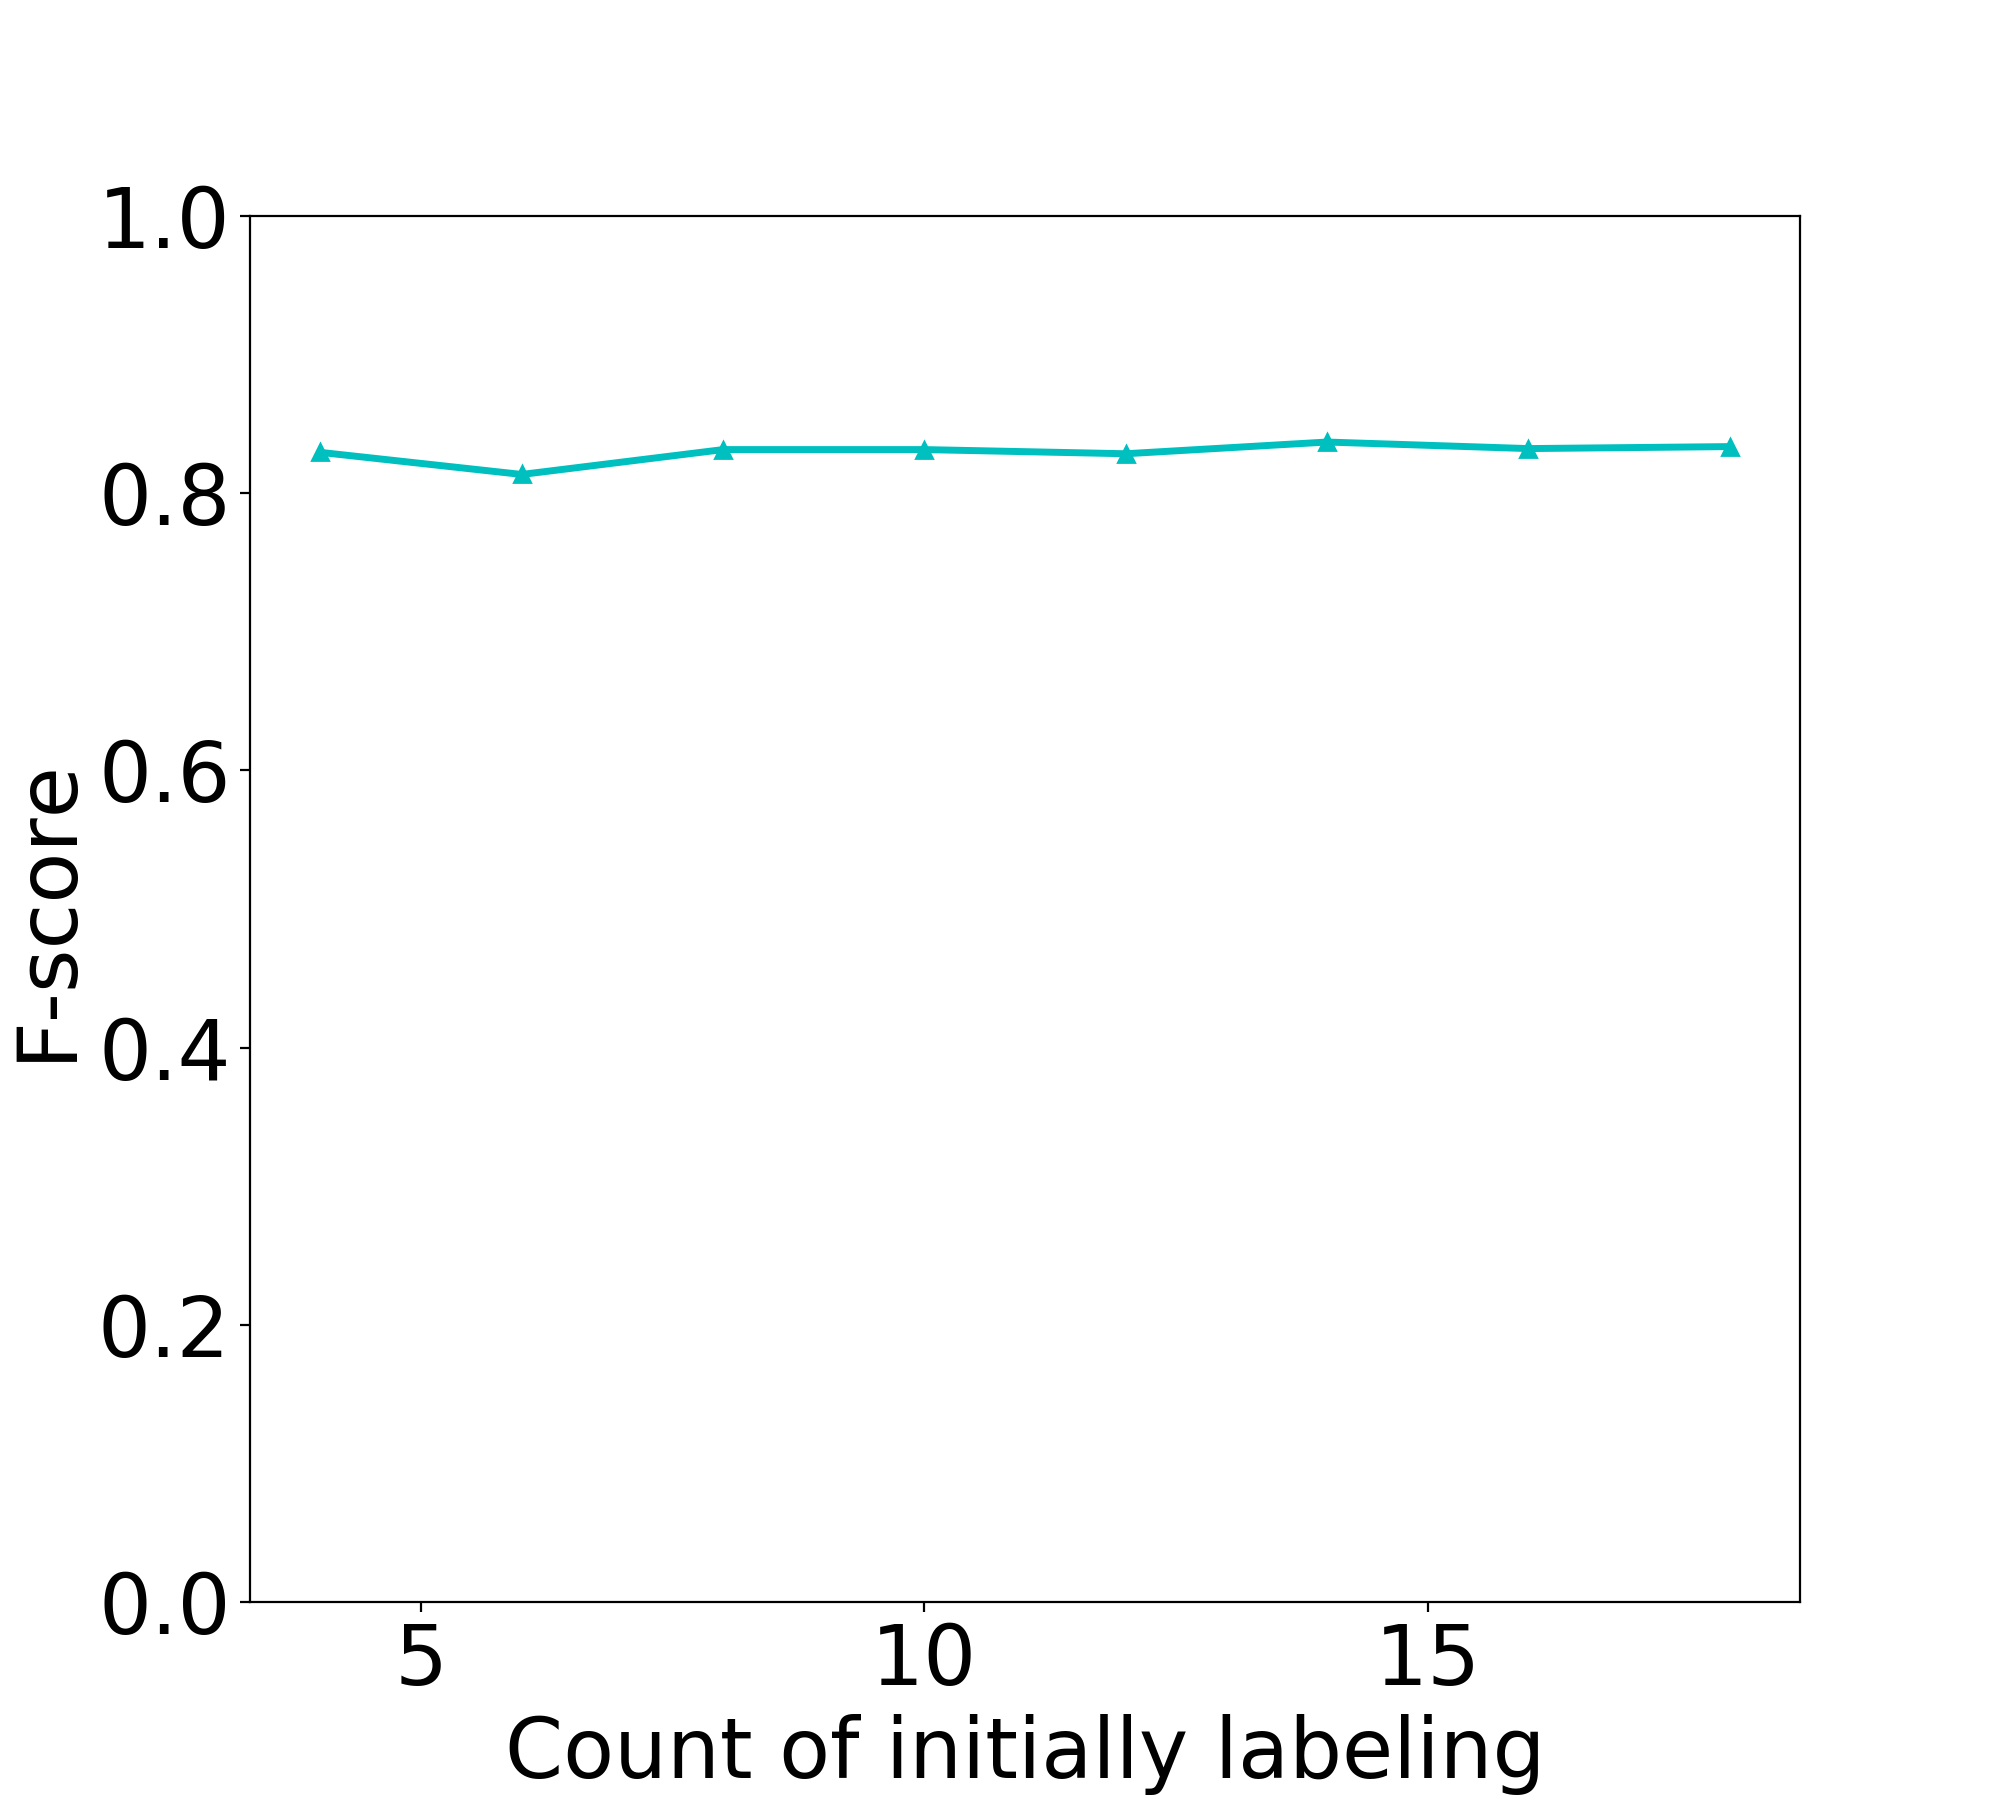
\includegraphics[width=1.1\linewidth]{ADS_Journal/PU figures/para_label_count.png}\label{c}
      \end{minipage}}
	  \caption{Comparison experiment of parameters.}
	  \label{fig:parameters} 
\end{figure}
